\documentclass[letterpaper]{article}
\usepackage[margin=1in]{geometry}
\usepackage[utf8]{inputenc}
\usepackage{textcomp}
\usepackage{amssymb}
\usepackage{natbib}
\usepackage{graphicx}
\usepackage{gensymb}
\usepackage{amsthm, amsmath, mathtools}
\usepackage[dvipsnames]{xcolor}
\usepackage{enumerate}
\usepackage{mdframed}
\usepackage[most]{tcolorbox}
\usepackage{csquotes}
% https://tex.stackexchange.com/questions/13506/how-to-continue-the-framed-text-box-on-multiple-pages

\tcbuselibrary{theorems}

\newcommand{\R}{\mathbb{R}}
\newcommand{\Z}{\mathbb{Z}}
\newcommand{\N}{\mathbb{N}}
\newcommand{\Q}{\mathbb{Q}}
\newcommand{\C}{\mathbb{C}}
\newcommand{\code}[1]{\texttt{#1}}
\newcommand{\mdiamond}{$\diamondsuit$}
\newcommand{\PowerSet}{\mathcal{P}}
\newcommand{\Mod}[1]{\ (\mathrm{mod}\ #1)}
\DeclareMathOperator{\lcm}{lcm}

%\newtheorem*{theorem}{Theorem}
%\newtheorem*{definition}{Definition}
%\newtheorem*{corollary}{Corollary}
%\newtheorem*{lemma}{Lemma}
\newtheorem*{proposition}{Proposition}


\newtcbtheorem[number within=section]{theorem}{Theorem}
{colback=green!5,colframe=green!35!black,fonttitle=\bfseries}{th}

\newtcbtheorem[number within=section]{definition}{Definition}
{colback=blue!5,colframe=blue!35!black,fonttitle=\bfseries}{def}

\newtcbtheorem[number within=section]{corollary}{Corollary}
{colback=yellow!5,colframe=yellow!35!black,fonttitle=\bfseries}{cor}

\newtcbtheorem[number within=section]{lemma}{Lemma}
{colback=red!5,colframe=red!35!black,fonttitle=\bfseries}{lem}

\newtcbtheorem[number within=section]{example}{Example}
{colback=white!5,colframe=white!35!black,fonttitle=\bfseries}{def}

\newtcbtheorem[number within=section]{note}{Important Note}{
        enhanced,
        sharp corners,
        attach boxed title to top left={
            xshift=-1mm,
            yshift=-5mm,
            yshifttext=-1mm
        },
        top=1.5em,
        colback=white,
        colframe=black,
        fonttitle=\bfseries,
        boxed title style={
            sharp corners,
            size=small,
            colback=red!75!black,
            colframe=red!75!black,
        } 
    }{impnote}
\usepackage[utf8]{inputenc}
\usepackage[english]{babel}
\usepackage{fancyhdr}
\usepackage[hidelinks]{hyperref}

\pagestyle{fancy}
\fancyhf{}
\rhead{Math 170B}
\chead{Monday, May 22, 2023}
\lhead{Lecture 22}
\rfoot{\thepage}

\setlength{\parindent}{0pt}

\begin{document}
\section{Descent Methods (Section 11.2)}
Recall the one-dimensional function $f: \R \mapsto \R$. If $f'(x)$ is available, then we seek $f'(x) = 0$.
\begin{center}
    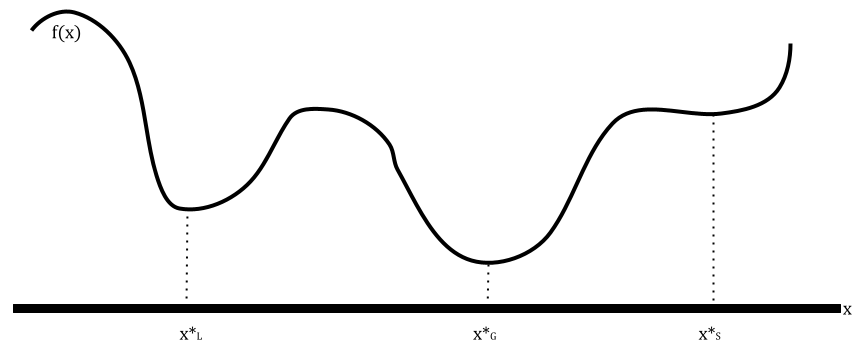
\includegraphics[scale=0.5]{../assets/1varopt_ex.png}
\end{center}
Newton's method is generally an effective method for finding the zeros of $f'(x)$. Also note, however, that we need $f''$; 
\[x_{k + 1} = x_{k} - \frac{f'(x_{k})}{f''(x_{k})}, \qquad k = 0, 1, 2, \hdots\]
We can also consider using methods like the bisection methods to find the zero. 

\subsection{Many Variables Walkthrough}
For many variables, we now have the function \[F: \R^m \mapsto \R.\] Note that the input is a vector of numbers $\vec{x} = \begin{bmatrix}
    x_1 \\ x_2 \\ \vdots \\ x_m
\end{bmatrix}$. The \textbf{gradient} of $F(x)$ is given by 
\[\nabla F(x) = g(x) = \begin{bmatrix}
    \frac{\partial F}{\partial x_1} \\ 
    \frac{\partial F}{\partial x_2} \\ 
    \vdots \\ 
    \frac{\partial F}{\partial x_m}
\end{bmatrix} \in \R^m.\] The gradient of the gradient, known as the \textbf{Hessian matrix}, is then given by 
\[\nabla^2 F(x) = H(x) = \begin{bmatrix}
    \frac{\partial^2 F}{\partial x_1 \partial x_1} & \frac{\partial^2 F}{\partial x_1 \partial x_2} & \hdots & \frac{\partial^2 F}{\partial x_1 \partial x_m} \\ 
    \frac{\partial^2 F}{\partial x_2 \partial x_1} & \frac{\partial^2 F}{\partial x_2 \partial x_2} & \hdots & \frac{\partial^2 F}{\partial x_2 \partial x_m} \\ 
    \vdots & \vdots & \ddots & \vdots \\ 
    \frac{\partial^2 F}{\partial x_m \partial x_1} & \frac{\partial^m F}{\partial x_m \partial x_2} & \hdots & \frac{\partial^2 F}{\partial x_m \partial x_m}\\ 
\end{bmatrix}.\]
It's typical to use 2 terms in a Taylor expansion $F(x_{k} + p)$, with $p \in \R^m$. So, \[F(x_k + p) = F(x_k) + p^T \nabla F(x_k) + \frac{1}{2} p^T \nabla^2 F(x_k) p + \hdots\]
How do we define the update $p$? Because, that way, we could do $x_{k + 1} = x_{k} + p$.

\subsection{Steepest Descent Method}
The goal of the steepest descent method is to make $p^T \nabla f(x_k) < 0$ as negative as possible. To do this, we'll consider any $p$ so $||p||_2 = 1.$ Then, by the Cauchy-Schwartz inequality, \[-||p||_2 \cdot ||\nabla f(x_k)||_2 \leq  p^T \nabla f(x_k) \leq ||p||_2 \cdot ||\nabla f(x_k)||_2.\]
Then, we're looking for 
\[p^T \nabla f(x_k) \geq -||p||_2 \cdot ||\nabla f(x_k)||_2 = -||\nabla f(x_k)||_2.\] From there, we have \[p = -\frac{\nabla f(x_k)}{||\nabla f(x_k)||_2}.\] Note that, in this case, $p$ is a multiple of the negative gradient, i.e., the sharpest descent direction. A line-search strategy to finding this $p$ is 
\[\min_{\alpha > 0} F(x_k - \alpha \nabla F(x_k)).\]

\subsubsection{Steepest Descent Algorithm}
The algorithm for steepest descent takes the following arguments: 
\begin{itemize}
    \item $x_0 \in \R^m$: the initial starting point. 
    \item $\epsilon > 0$: the tolerance.
    \item $M$: the maximum number of iterations.
\end{itemize}

\begin{algorithm}[H]
    \caption{Steepest Descent}
    \begin{algorithmic}[1]
        \Function{Steepest}{$x_0, \epsilon, N$}
            \State $k \gets 0$
            \While{$||\nabla f(x_k)||_2 > \epsilon$ and $k \leq M$}
                \State $\alpha_k \gets \min_{\alpha} F(x_{k} - \alpha \nabla F(x_{k}))$
                \State $x_{k + 1} \gets x_k - \alpha \nabla F(x_k)$
                \State $k \gets k + 1$
            \EndWhile 
        \EndFunction
    \end{algorithmic}
\end{algorithm}
\textbf{Remarks:}
\begin{itemize}
    \item This algorithm doesn't check if the point that's found is a minimum.
    \item This algorithm may ``zig-zag.'' 
\end{itemize}
With this in mind, we now think about the directional derivative of $F(x_{k} + \alpha p)$. In particular, note that \[0 = F'(x_k + \alpha p)|_{\alpha = \alpha k} = p^T \nabla F(x_k + \alpha_k p) = p^T \nabla F(x_{k + 1}).\] 
In steepest descent, $p = -\nabla F(x_k)$, so \[0 = -\nabla F(x_{k})^T \nabla F(x_{k + 1}).\]

\begin{mdframed}
    (Example: Test Function.) Consider Rosenbrock's function \[F(x) = 100 (x_1^2 - x_2)^2 + (1 - x_1)^2,\] with the starting point being $x = \begin{bmatrix}
        -1.2 \\ 1.0
    \end{bmatrix}$. 
    
    \bigskip 

    Additionally, consider Powell's Singular Function, 
    \[F(x) = (x_1 + 10x_2)^2 + 5(x_3 - x_4)^2 + (x_2 - 2x_3)^4 + 10(x_1 - x_4)^4,\] 
    with starting point $x = \begin{bmatrix}
        3 \\ -1 \\ 0 \\ 1
    \end{bmatrix}.$
\end{mdframed}
We have two main strategies to determine iterates: 
\begin{enumerate}
    \item Line search. 
    \begin{itemize}
        \item Fix direction $p$. 
        \item Determine step length $\alpha_k = \min_{\alpha > 0} F(x_k + \alpha p)$.
    \end{itemize}

    \item Trust-Region  
    \begin{itemize}
        \item Fix step length $\Delta_k > 0$.
        \item Determine direction $p$, \[\min_{||p|| \leq \Delta_k} \left(F_{k} + p^T \nabla F_k +  \frac{1}{2}p^T B_k p\right).\] 
        Note that $B_k \in \R^{m \times m}$ is a Hessian $H(x_k)$, or an approximation to it.
    \end{itemize}
\end{enumerate}

\end{document}